%!TEX root = *.tex
%%%%%%%%%%%%%%%%%%
% カウンタのリセット
\setcounter{figure}{0}
% 問題文
気体を容器に封入したとき,気体分子は容器の壁面と繰り返し衝突をしている.
図1のように,1辺の長さが\mbox{$L\unit{m}$}の立方体の容器に分子1個の質量が\mbox{$m\unit{kg}$}の単原子分子理想気体が$N$個入っている.
この気体から\z 軸に垂直な壁面Aが受ける圧力を考える.
容器内の気体の温度は\mbox{$T\unit{K}$}で一定であり,分子どうしの衝突は無視する.
アボガドロ定数を\mbox{$N_{\rm A}\textup{〔mol}^{-1}\textup{〕}$},
気体定数を$R\text{〔J/}(\text{mol}\cdot \text{K})\text{〕}$,
重力加速度の大きさを\mbox{$g$\text{〔m/}$\text{s}^2$\text{〕}}とする.
次の文章中の\BrankNo{ア}~\BrankNo{セ}に適切な数式または数値を入れよ.



\hang{(1)}
初めに重力が作用していない場合について考える.
ある1個の分子の\z 軸方向の速度の成分を$v_z\unit{m/s}$とすると,
分子が壁面Aと弾性衝突したときに壁面Aが分子から受ける力積は\BrankNo{ア}$\textup{〔N}\cdot\textup{s〕}$である.
分子が壁面Aと衝突から次に壁面Aと衝突するまでの時間は\BrankNo{イ}$\unit{s}$であるため,分子は時間$\Delta t\unit{s}$の間に,壁面Aと\BrankNo{ウ}回衝突する.
したがって,時間$\Delta t$の間に壁面Aが受ける力積は\BrankNo{エ}$\textup{〔N}\cdot\textup{s〕}$となり,
1個の分子によって壁面Aが受ける力$f$は\BrankNo{オ}$\times {v_z}^2\unit{N}$と\z 軸における速度成分の2乗${v_z}^2$を用いて表せる.
$N$個の分子によって壁面Aが受ける力$F\unit{N}$については,すべての分子は不規則に運動しており,
速度成分の2乗平均はどの成分についても等しいので,$N$個の分子の速度の2乗平均$\overline{v^2}$〔$\text{m}^2$/$\text{s}^2$〕を用いて\BrankNo{カ}と表せる.
以上から,圧力は\BrankNo{キ}〔N/$\text{m}^2$〕となる.
また,状態方程式から$\overline{v^2}$は$m,\,N_A,R,T$を用いて\BrankNo{ク}となり,
気体の内部エネルギー$U\unit{J}$は$N,N_A,R,T$を用いて\BrankNo{ケ}となることがわかる.

\hang{(2)}
\z 軸の負の向きに一様な重力が作用する場合,容器内の気体の密度と圧力に勾配が生じる.
図2のように,容器の底からはかった高さを$z\unit{m}$とし,高さ\z における気体の圧力を$P(z)$〔N/$\text{m}^2$〕,密度を$d(z)$〔kg/$\text{m}^3$〕とする.
\z から$\Delta z$だけ高いところを$(z+\Delta z)\unit{m}$とし,高さ\z における厚さ$\Delta z$,断面積$L^2$の気柱について考えると,
高さ$(z+\Delta z)$における気体の圧力$P(z+\Delta z)$〔N/$m^2$〕は,気柱内における気体の密度の勾配が無視できるほど$\Delta z$が小さいとき,
$P(z),\,d(z),\,\Delta z$などを用いて\BrankNo{コ}と近似できる.
また,容器内の気体は単原子分子理想気体であるため,$d(z)$は$P(z)$と$T$などを用いて\BrankNo{サ}と表せる.
以上から,気体1\,mol\,あたりの質量が$4.0\times 10^{-3}\,\text{kg}/\text{mol}$,
温度が300\,K\,であるとき,$P(z+\Delta z)$が$P(z)$と比べて$0.010\%$だけ小さくなるような高さの差は,
$R=8.3\,\text{〔J/}(\text{mol}\cdot \text{K})\text{〕}$,
$g=9.8$\,\text{〔m/}$\text{s}^2$\text{〕}とすると,
有効数字2桁で\BrankNo{シ}mと見積もることができる.
また,容器の底における気体の圧力と密度をそれぞれ$P(0)$\,〔N/$\text{m}^2$〕,
$d(0)$\,〔kg/$\text{m}^3$〕,高さ$L$における気体の圧力と密度をそれぞれ$P(L)$\,〔N/$\text{m}^2$〕,$d(L)$\,〔kg/$\text{m}^3$〕とすると,$P(0)$と$P(L)$との差は$N,\,m,\,g,\,L$を用いて\BrankNo{ス}となり,
$d(0)$と$d(L)$との差は$N_{\rm A},\,m,\,g,\,L,\,R,\,T$を用いて\BrankNo{セ}となる.

\begin{figure}[H]
  \centering
  \begin{minipage}{.3\columnwidth}
    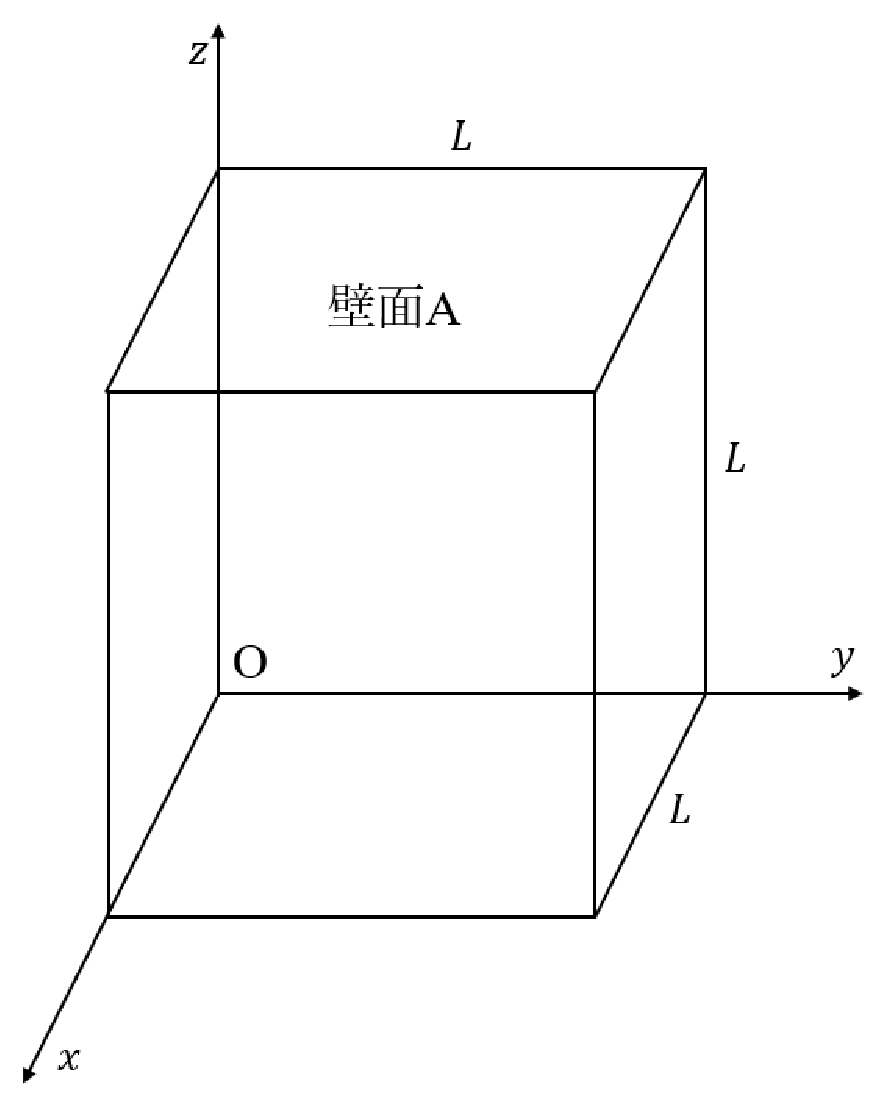
\includegraphics[width=\columnwidth]{../graphs/jumon_65_1.eps}
    \caption{}
  \end{minipage}
  \begin{minipage}{.3\columnwidth}
    \centering
    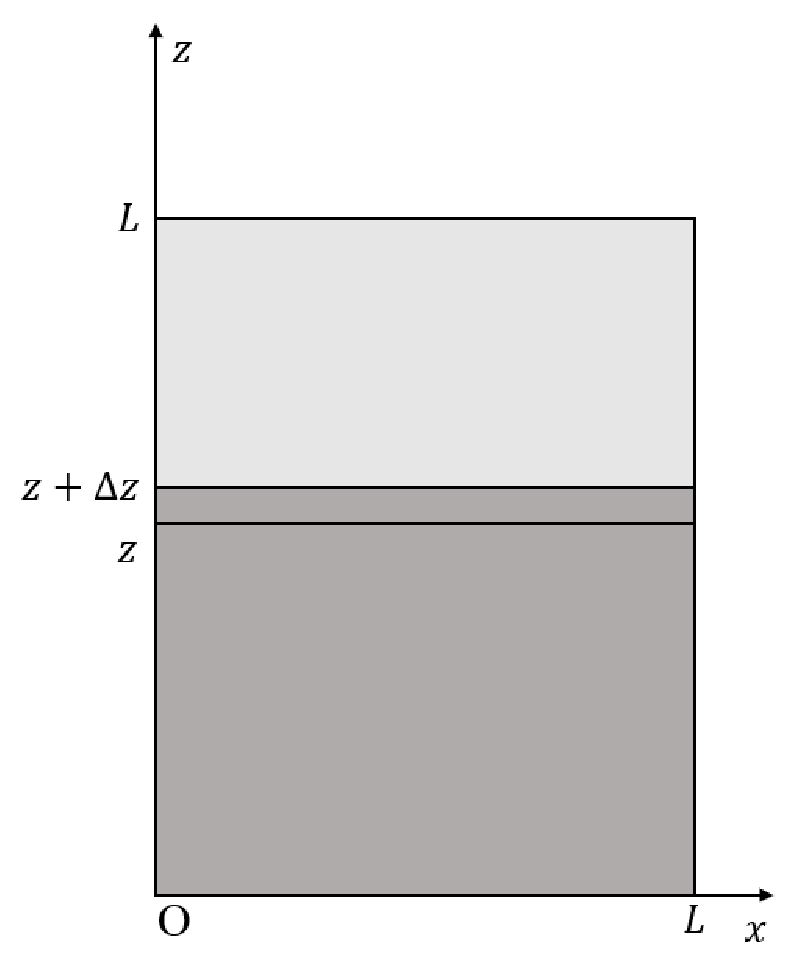
\includegraphics[width=\columnwidth]{../graphs/jumon_65_2.eps}
    \caption{} 
  \end{minipage}
\end{figure}


% メモ
\begin{comment}

\end{comment}


%%%%%%%%%%%%%%%%%%
